%!TEX root = ../main.tex
\documentclass[../main.tex]{subfiles}
\begin{document}
  \chapter{Method}\label{chapter:method}
  This chapter outlines the method used to construct a finite difference scheme for the deterministic Jump Growth Equation, \autoref{eq:mvf:diffusion}. It begins with a discussion about the steady state of the McKendrick-von Foerster Equation and how this helps to solve the Jump Growth Equation. Following this we apply the mathematics in \autoref{chapter:fdes} and \cite{rosinger2008} to construct a finite difference scheme that is stable and consistent, and thus convergent.


  \section{Steady State Solutions}\label{sec:met:steadystate}
  In marine ecosystems it's been found that the abundance of organisms within weight classes is roughly constant (\cite{sheldon1972}) if those weight classes are distributed logarithmically. Further, averaged over time, this abundance changes rather little (\cite{datta2011}) suggesting that the system is near steady state. \cite{benoit2004} found that the McKendrick-von Foerster Equation has a power law steady steady state of the form $\phi(w) \propto w^{\gamma}$. We combine this reasearch to now show that the the McKendrick-von Foerster Equation with diffusion (\autoref{eq:mvf:diffusion}) can be transformed using the logarithmic change of variables and appropriate change of function to have a constant solution if the work of \cite{benoit2004} is correct.

  It first helps to transform to a dimensionless variable $x = \log{w}$, with $\varphi(x) \mathrm{d}x = \phi(w) \mathrm{d}w$ which we will show makes our equations behave much more nicely under translation. Following the method found in \autoref{app:sec:cov} we can change variables from our weight indexed equation
  \begin{equation}
    u_t = -(g \cdot u)_w - \mu \cdot u + \frac{1}{2}(D \cdot u)_{xx}
  \end{equation}
  to a dimensionless equation for $\rho(x) = \e{(1 - \gamma) \log{w}} u(w)$,
  \begin{equation}
    \e{\gamma x} \rho_t = - (\bar{g} \rho)_x - \bar{\mu} \e{\gamma x} \rho + \frac{\e{-x}}{2} \left( (\bar{D} \rho)_{xx} - (\bar{D} \rho)_x \right),
  \end{equation}

  for the coefficient functions $\bar{g}, \bar{\mu}, \bar{D}$ found in \autoref{app:sec:cov}. Through this transform and the knowledge from \autoref{sec:met:steadystate} we find that at steady state $\rho(x) \propto 1$ and so if $u(w) = u_0 w^{\gamma}$ then $\rho(x) = u_0$ which is much easier to run tests against since for a initial condition which consists of a small perturbation $\epsilon(x)$ we can much more easily see if the system returns to a steady state.

  \section{Coefficient Observations}
  We first observe that under the logarithmic weight index that $\bar{S}(x)$ is a gaussian curve which we will say takes the form defined in \autoref{eq:mvf:feedgaussian}. Thus under the coefficient functions $\bar{S}(x - x')$ takes the form
  \begin{equation}
    \bar{S}(x - x') = C \exp{\left( -\frac{(x - x' - \beta)^2}{2 \sigma^2} \right)} = C \exp{\left( -\frac{(x' - (x - \beta))^2}{2 \sigma^2} \right)},
  \end{equation}

  where $C = (2 \sigma ^2 \pi)^{-1}$, and again this takes the form of a Gaussian centered at $x - \beta$. Further if $Gau_{\beta, \sigma}(x)$ is a Gaussian then by completing the square it is easy to see that
  \begin{equation}
    \e{\gamma x} Gau_{\beta, \sigma}(x) \propto Gau_{\lambda, \eta}(x).
  \end{equation}

  If, for a simple test, we take $\rho$ to be at the steady state and thus constant $\rho(x) = \upsilon_0$ and consider the growth coefficient $\bar{g}(x)$ then
  \begin{equation}
    \bar{g}(x) = \upsilon_0 K \int \e{(\gamma + 1) x'} \bar{S}( x - x' ) \: \mathrm{d} x'.
  \end{equation}

  Considering the inner function we just said that this will take the form of a Gaussian curve for various $x$, and this can be numerically validated using a simple MATLAB script (See \autoref{fig:met:gaussian}). However as can be seen on the the red curve and partially on the yellow curve for this range of $x$ we see that much of the Gaussian curve is cut off and thus, if this was to be integrated would be missing much of the area.

  \begin{figure}[ht]
    \centering
    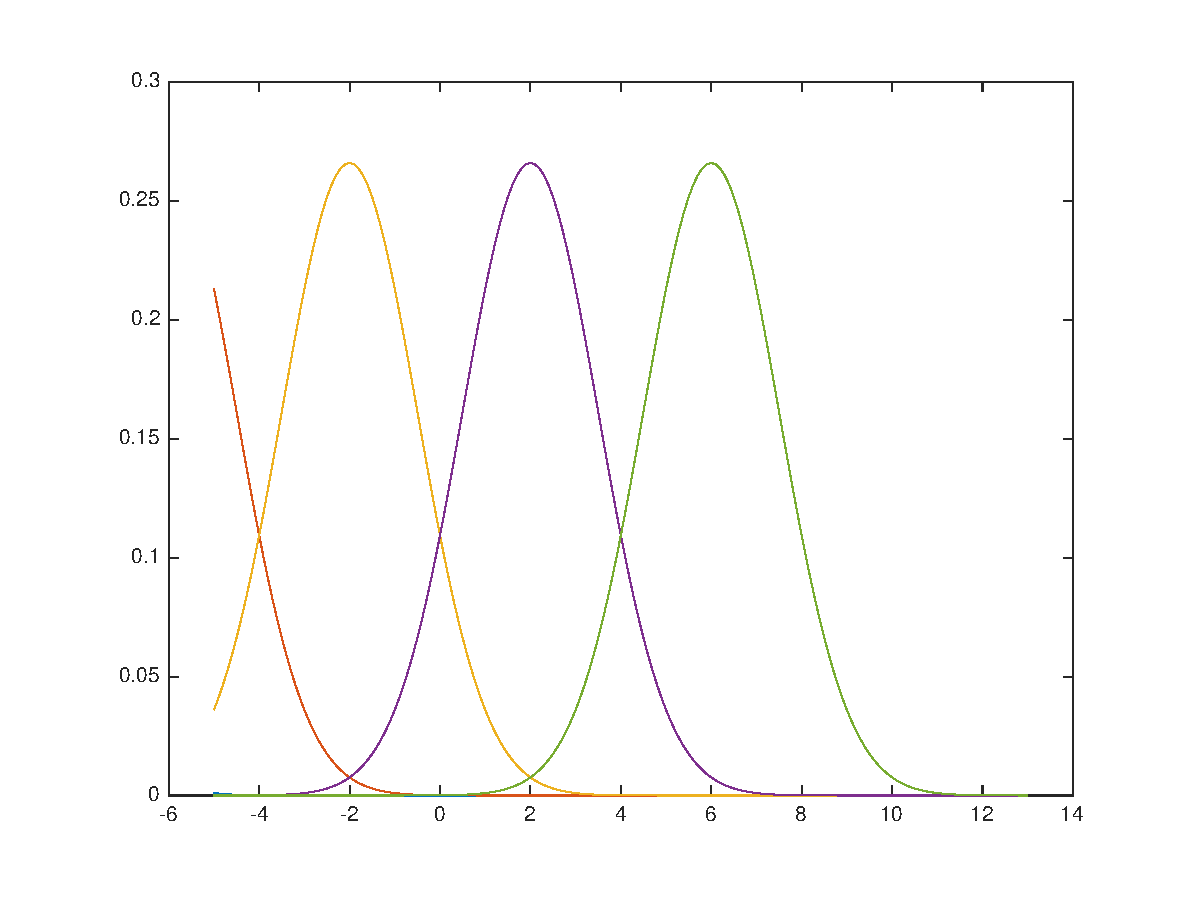
\includegraphics[width=0.5\textwidth]{img/kernelExample.eps}
    \caption{Numerical validation that the integrand for the growth coeffient takes a Gaussian form if $\rho$ is at steady state. \label{fig:met:gaussian}}
  \end{figure}

\end{document}
